\section{Classification des aéronefs}
Un \gls{aéronef} \anglais{aircraft} est un appareil capable de s'élever et de se mouvoir au sein de l'atmosphère terrestre. On divise les aéronefs en 2 grandes familles :
\begin{itemize}
	\item les  \gls{aérostat}s \anglais{aerostat/lighter-than-air aircraft}, qui sont des appareils plus légers que l'air,
	\item les  \gls{aérodyne}s \anglais{heavier-than-air aircraft}, qui sont plus lourds que l'air.
\end{itemize}

Dans cette partie, nous étudierons les aéronefs mais également les engins spatiaux. Ceux ci ne peuvent être qualifiés d'aéronefs, car, bien que certains d'entre eux puissent se déplacer dans l'atmosphère, ils peuvent également se mouvoir en dehors de celle-ci.

\subsubsection{Pourquoi classer les aéronefs ?}
Chaque type d'aéronef dispose de propriétés et de contraintes qui lui sont propres. La classification des aéronefs en grand groupes présentant des caractéristiques communes permet de leur associer aisément des notions réglementaires (licence de pilote nécessaire, minima météo, zone de vol autorisées...), techniques (fréquences et mode d'entretien, contraintes de conception) ou administratives (immatriculation, assurance...).

\subsection{Aérostats}
	\subsubsection{Montgolfière}
	La montgolfière \anglais{hot air balloon} est un aérostat gonflé à l'air chaud. \\
	
	Elle est composé d'un ballon (appelé enveloppe) sous lequel est accroché une nacelle dans laquelle prennent place les passagers et le pilote nommé aérostier. Un bruleur généralement alimenté au gaz permet de chauffer l'air contenu dans le ballon. Le pilote chauffe l'air à l'aide du bruleur pour faire monter la montgolfière. \\
	
	La montgolfière ne dispose d'aucun moyen pour se diriger, elle est entièrement soumise aux vents pour ses déplacements. Cependant, le pilote peut exploiter les variation de sens du vent aux différentes altitudes pour orienter son vol dans une certaine mesure.
	
	\begin{figure}[H]
  	\centering
    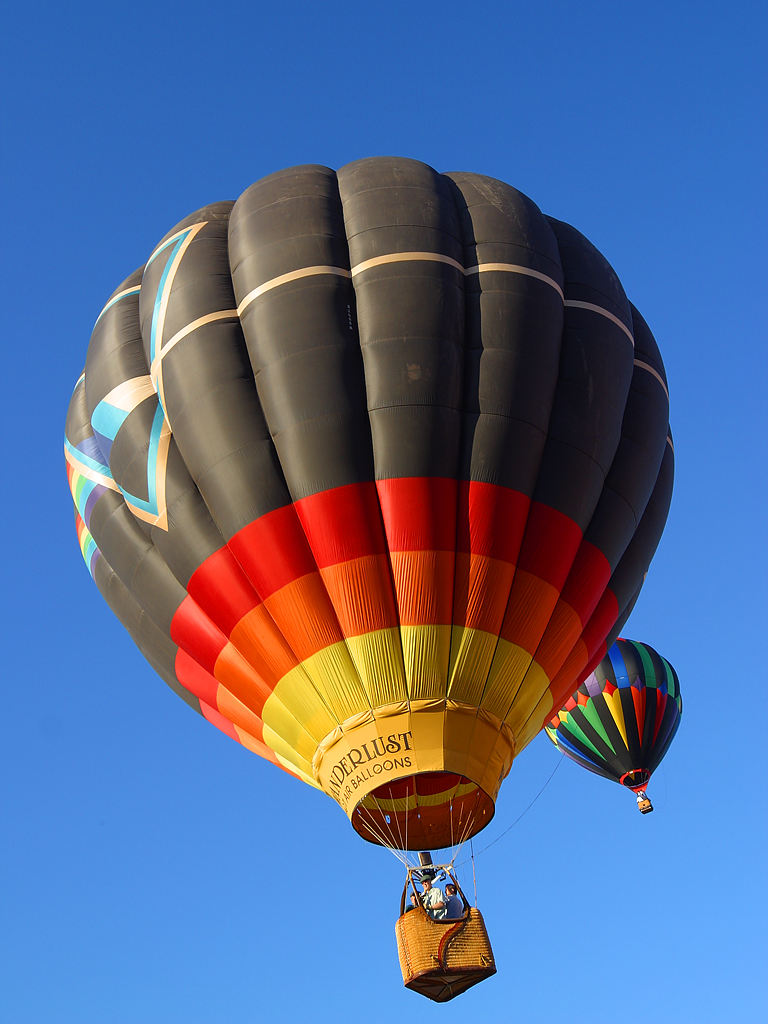
\includegraphics[width=0.4\textwidth]{1-EtudeAeronefs/img/montgolfiere.jpg}
  	\caption{2 ballons dirigeables \cite{img:montgolfiere}}
	\end{figure}	
	
	\histoire{La montgolfière a été le premier aéronef conçu par l'humain. Les frères Montgolfier ont conçu le premier ballon à air chaud et réalisé le premier vol en 1783. La même année, ils font voler des animaux puis Jean-François \textbf{Pilâtre de Rozier} et le Marquis d'Arlandes réalisent le premier vol libre humain. \\ \\ En 1785, Jean-Pierre Blanchard effectue la première traversée de la manche avec un aéronef, 124 ans avant celle effectuée par Louis Blériot en avion.}
	\subsubsection{Ballon à gaz}
	Le ballon à gaz \anglais{gas balloon} est gonflé avec un gaz plus léger que l'air (hydrogène ou hélium).	
	
	\subsubsection{Dirigeable}
	Le dirigeable \anglais{airship} ou ballon dirigeable est un ballon à gaz équipés d'une systèmes propulsifs lui permettant de se diriger (aussi bien sur le plan horizontal que vertical). \\
	
	Les premiers dirigeables étaient gonflés à l'hydrogène. Ce gaz est dangereux car très inflammable. Les dirigeables modernes sont désormais gonflés à l'hélium. L'hélium est un gaz sur car ininflammable, mais il est plus cher et plus lourd que l'hydrogène (un ballon à l'hélium nécessitera une enveloppe plus grande qu'un ballon à hydrogène de même capacité).
	
	\begin{figure}[H]
  	\centering
    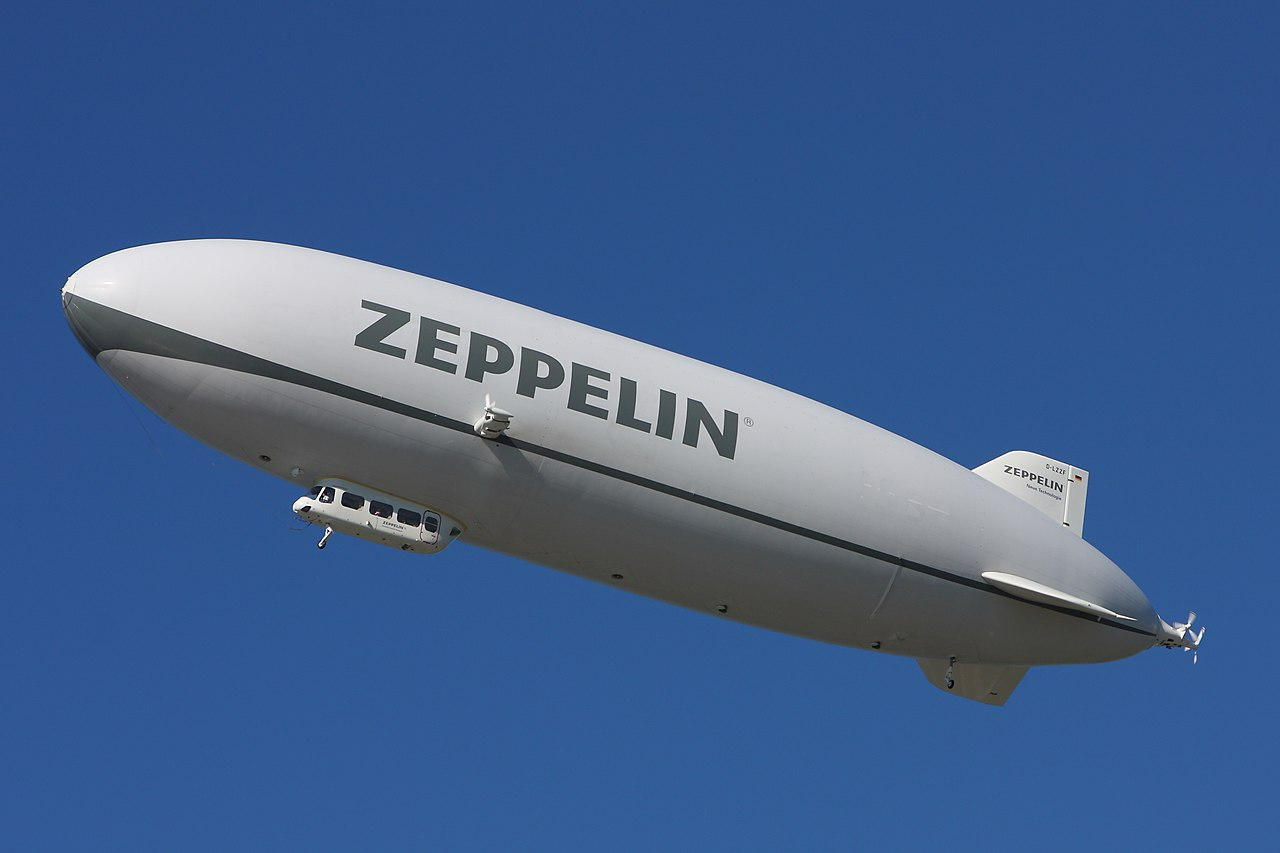
\includegraphics[width=0.4\textwidth]{1-EtudeAeronefs/img/dirigeable.jpg}
  	\caption{Un dirigeable moderne \cite{img:dirigeable}}
	\end{figure}	

\subsection{Aérodynes}
	\subsubsection{Aéronef à voilure fixe}
		Les appareils à voilure fixe \anglais{fixed-wing aircraft}, également appelés aéroplanes sont des aéronefs dont la sustentation est assurée par des surfaces fixes (ailes). Ce type d'aéronef ne peut se maintenir en l'air que si un flux d'air suffisant existe sur ses ailes.

		\paragraph{Avions}
		L'avion est un aérodyne dont la sustentation est assurée par le défilement du flux d'air sur ses ailes. La vitesse est apportée par un organe propulsif (moteur via une hélice, réacteur, moteur fusée...).
	
		\paragraph{Planeurs}
		
	\subsubsection{Aéronef à voilure tournante}
	Les appareils à voilure tournante \anglais{rotary-wing aircraft}, également appelés aérogires, sont des aéronefs dont la sustentation est assurée par la rotation d'un ou plusieurs rotors.
		\paragraph{Hélicoptères}
		\paragraph{Autogyre}
		\paragraph{Convertible}
		
	\subsubsection{Aéronef à voilure souple}
	Les aéronefs à voilure souple \anglais{flexible wings} regroupe des aéronefs dont la voilure est généralement gonflée par l'air : parapente, paramoteur, parachute sportif moderne... Les deltaplanes rentrent également dans cette catégorie.
	
\subsection{Engins spatiaux}
	\subsubsection{Lanceurs}
		\paragraph{Fusées}
		\paragraph{Navettes spatiales}
		
	\subsubsection{Engins spatiaux}
		\paragraph{Satellites}
		\paragraph{Sondes}
		
\subsection{Les ULM}

Les \acrshort{ulm} (\acrlong{ulm}) \anglais{ultralight aircraft} sont un ensemble d'aéronefs motorisés de faible masse. De part cette caractéristique, ils bénéficient de facilités quant à leurs conditions de conception et d'entretien. L'obtention d'une licence de pilote ULM est également simplifiée par rapport aux licences pour des appareils plus lourds. \\

Il existe une grande diversités d'ULM. Il est ainsi possible de piloter des ULM aérostats ou aérondynes, à voilures fixes, tournantes ou souples. En France, ils sont classés en 6 catégories \\


	\begin{figure}[H]
  	\centering
    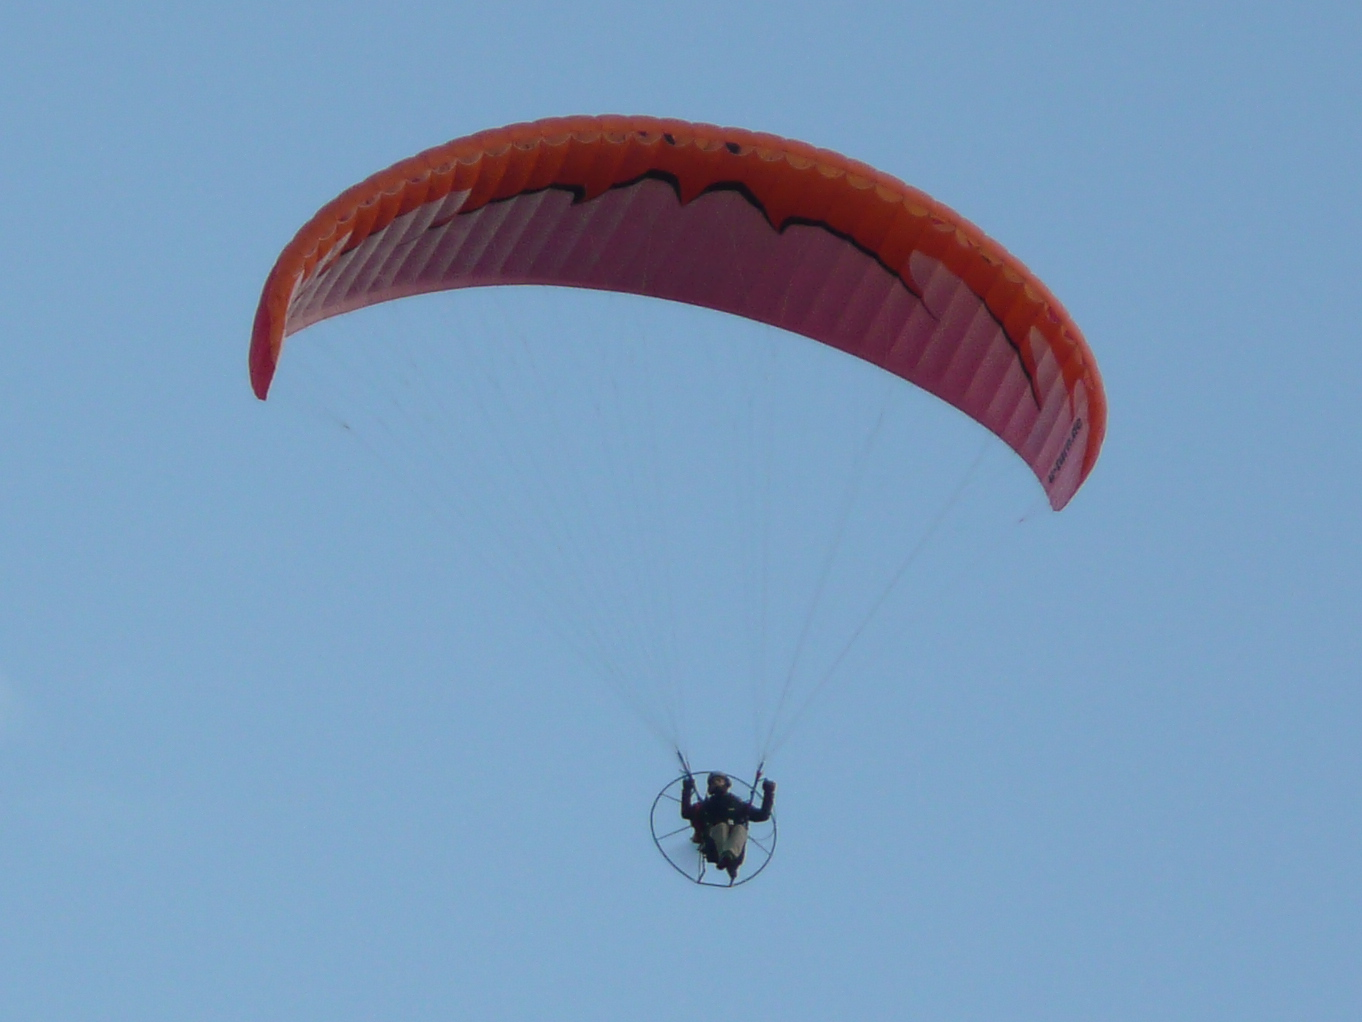
\includegraphics[width=0.4\textwidth]{1-EtudeAeronefs/img/ULM_Classe_1.jpg}
  	\caption{ULM classe 1 \cite{img:ulmClasse1}}
	\end{figure}	
	
	\begin{figure}[H]
  	\centering
    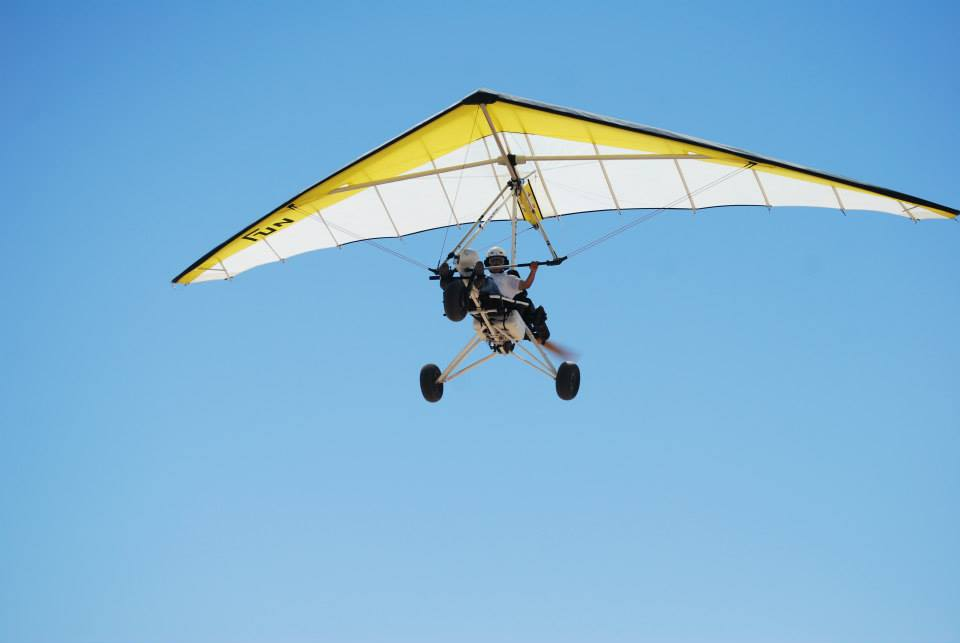
\includegraphics[width=0.4\textwidth]{1-EtudeAeronefs/img/ULM_Classe_2.jpg}
  	\caption{ULM classe 2 \cite{img:ulmClasse2}}
	\end{figure}	

	\begin{figure}[H]
  	\centering
    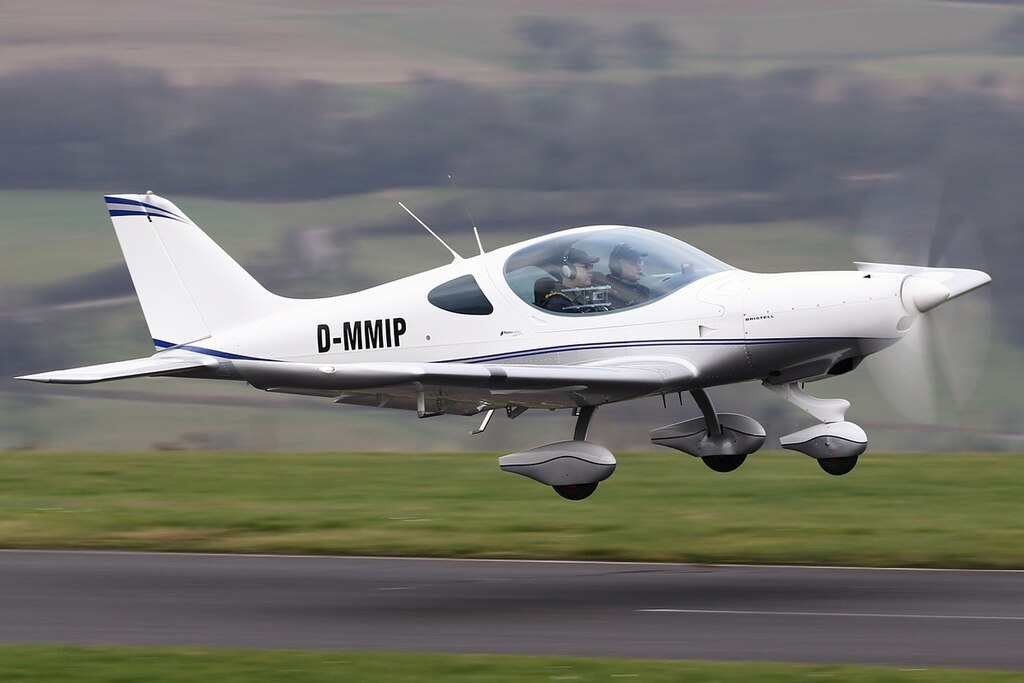
\includegraphics[width=0.4\textwidth]{1-EtudeAeronefs/img/ULM_Classe_3.jpg}
  	\caption{ULM classe 3 \cite{img:ulmClasse3}}
	\end{figure}	

	\begin{figure}[H]
  	\centering
    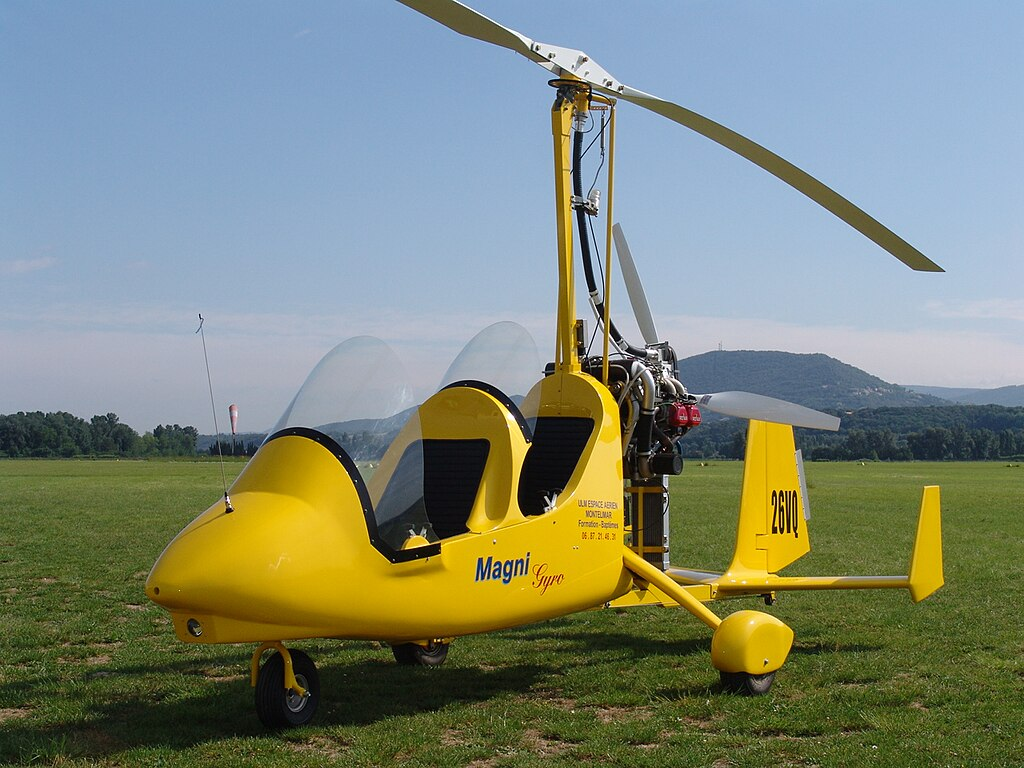
\includegraphics[width=0.4\textwidth]{1-EtudeAeronefs/img/ULM_Classe_4.jpg}
  	\caption{ULM classe 4 \cite{img:ulmClasse4}}
	\end{figure}	
	
	\begin{figure}[H]
  	\centering
    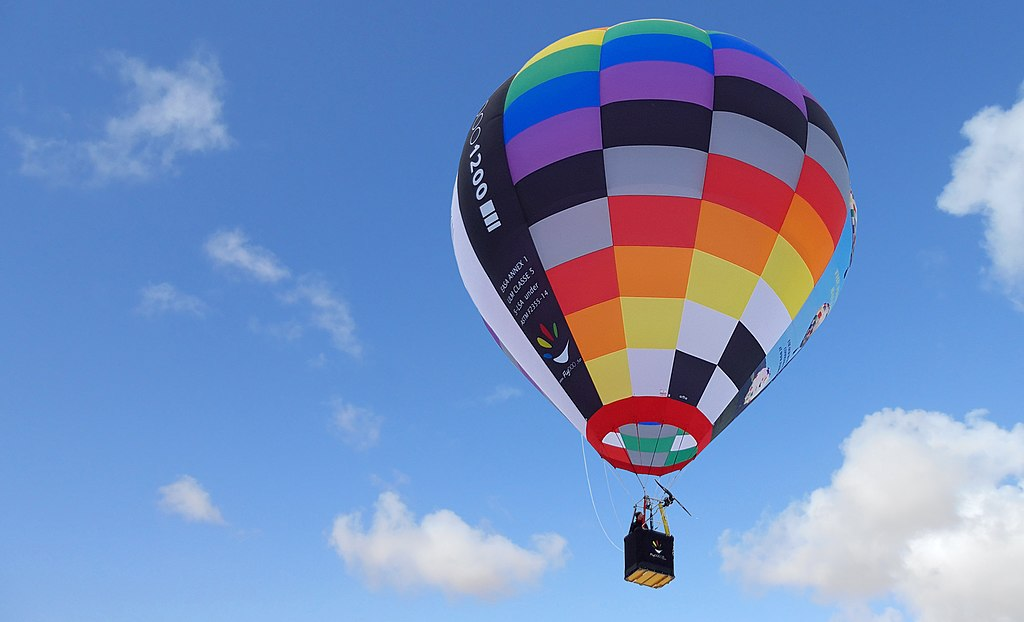
\includegraphics[width=0.4\textwidth]{1-EtudeAeronefs/img/ULM_Classe_5.jpg}
  	\caption{ULM classe 5 \cite{img:ulmClasse5}}
	\end{figure}	
	
	\begin{figure}[H]
  	\centering
    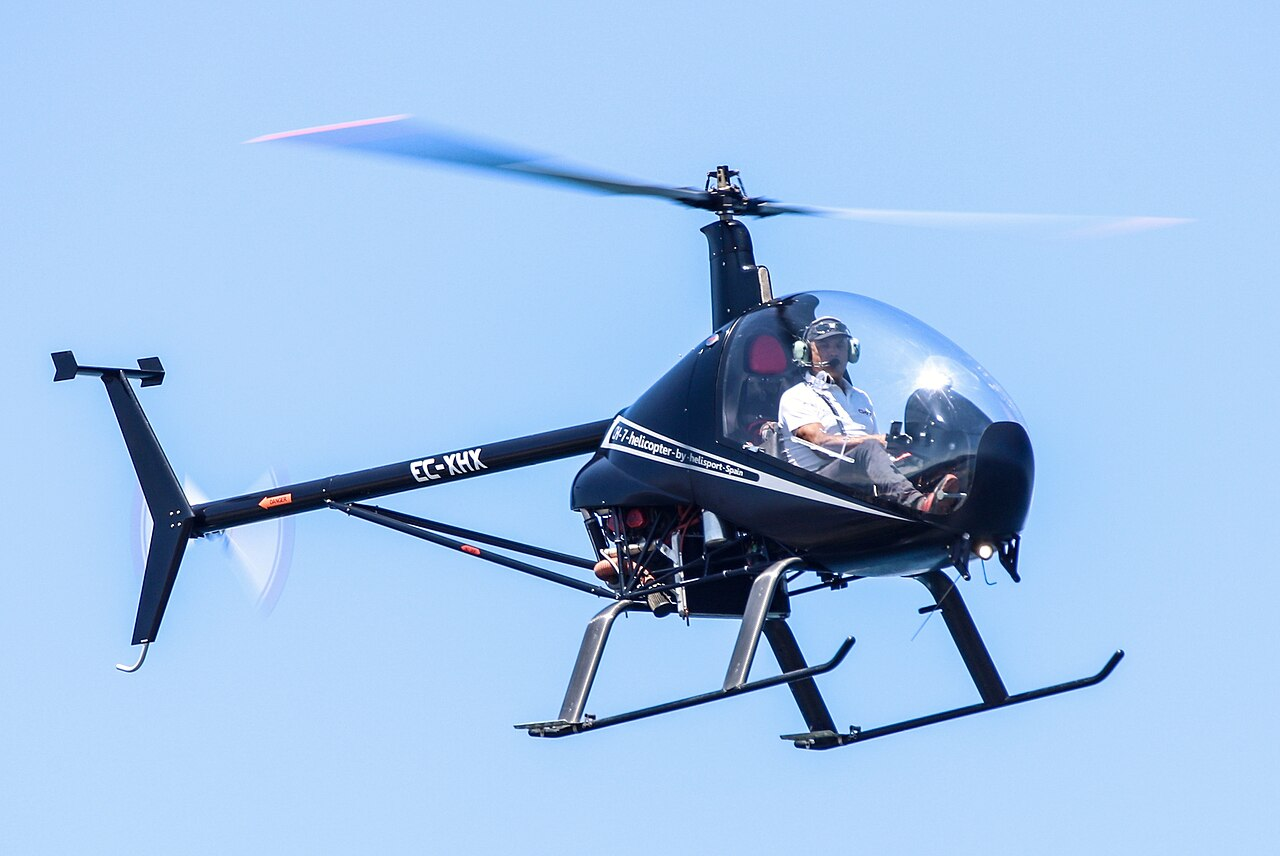
\includegraphics[width=0.4\textwidth]{1-EtudeAeronefs/img/ULM_Classe_6.jpg}
  	\caption{ULM classe 6 \cite{img:ulmClasse6}}
	\end{figure}


\subsection{Les drones}